% TEMPLATE for Usenix papers, specifically to meet requirements of
%  USENIX '05
% originally a template for producing IEEE-format articles using LaTeX.
%   written by Matthew Ward, CS Department, Worcester Polytechnic Institute.
% adapted by David Beazley for his excellent SWIG paper in Proceedings,
%   Tcl 96
% turned into a smartass generic template by De Clarke, with thanks to
%   both the above pioneers
% use at your own risk.  Complaints to /dev/null.
% make it two column with no page numbering, default is 10 point

% Munged by Fred Douglis <douglis@research.att.com> 10/97 to separate
% the .sty file from the LaTeX source template, so that people can
% more easily include the .sty file into an existing document.  Also
% changed to more closely follow the style guidelines as represented
% by the Word sample file. 

% Note that since 2010, USENIX does not require endnotes. If you want
% foot of page notes, don't include the endnotes package in the 
% usepackage command, below.

% This version uses the latex2e styles, not the very ancient 2.09 stuff.
\documentclass[letterpaper,twocolumn,10pt]{article}
\usepackage{usenix,epsfig}
\usepackage{times}  
\usepackage{epsfig}
\usepackage[TABBOTCAP]{subfigure}
\usepackage{tabularx}
\usepackage{graphicx} 
\usepackage{color}
\usepackage{xspace}
\usepackage{thumbpdf}
\usepackage{listings}
\usepackage{verbatim}
\usepackage{hyperref}
\usepackage{booktabs}
\usepackage{colortbl}
\usepackage[inline]{aplcomments}
\usepackage{inconsolata}
\usepackage{paralist}
\usepackage{xspace}
\usepackage{listings}
\lstset{
  basicstyle=\ttfamily,
  mathescape
}

\newcommenter{ak}{1.0,1.0,0.3}
\newcommenter{ac}{0.4,1.0,1.0}
\newcommand{\pktlanguage}{Domino\xspace}
\newcommand{\absmachine}{Banzai\xspace}
\newcommand{\tester}{Jayhawk\xspace}
\begin{document}

%don't want date printed
\date{}

%make title bold and 14 pt font (Latex default is non-bold, 16 pt)
%\title{\Large \bf Wonderful : A Terrific Application and Fascinating Paper}
\title{}

%for single author (just remove % characters)
\author{}
% copy the following lines to add more authors
% \and
% {\rm Name}\\
%Name Institution
%} % end author

\maketitle

% Use the following at camera-ready time to suppress page numbers.
% Comment it out when you first submit the paper for review.
%\thispagestyle{empty}

\subsection*{Abstract}
Data-plane algorithms execute on every packet traversing a network switch; they
encompass many schemes for congestion control, scheduling, network measurement,
active-queue management, security, and load balancing. Because these algorithms
are implemented in hardware today, they cannot be changed after being built. To
address this problem, recent work has proposed designs for programmable
line-rate switches.  However, these chips have only been used to program
stateless data-plane tasks, such as packet forwarding and access control. By
contrast, many data-plane algorithms create and modify algorithmic state on a
as part of their packet processing.

This paper presents \pktlanguage, a C-like imperative language to express
data-plane algorithms. \pktlanguage introduces the notion of a {\em packet
transaction}, defined as a sequential code block that is atomic and isolated
from other such code blocks.  The \pktlanguage compiler compiles \pktlanguage
code to \absmachine, a family of machine models based on emerging
programmable switch chipsets. We evaluate \pktlanguage by first designing
concrete \absmachine machines that support a variety of data-plane algorithms
with modest die area overhead. We then show how \pktlanguage simplifies
programming them, relative to current languages for programmable switches.

\section{Introduction}
\label{s:intro}

Data-plane algorithms~\cite{cestan} are algorithms that are implemented within
a network switch. These algorithms process every data packet that passes
through the switch, transforming the packet and often also some state stored on
the switch.  Examples of such algorithms include congestion-control that uses
feedback from switches~\cite{xcp, rcp, pdq, dctcp}, active queue
management~\cite{codel}, network measurement~\cite{opensketch, bitmap_george,
elephant_george}, and load-balanced routing in the data plane~\cite{conga}.

Because data-plane algorithms process every packet, an important implementation
requirement is the ability to process packets at line rate.  Consequently,
these algorithms are primarily implemented using dedicated hardware. However,
hardware designs are rigid, making it difficult to experiment with new
algorithms.

This rigidity affects network switch vendors that build network
equipment~\cite{cisco_nexus, dell_force10, arista_7050} based on
merchant-silicon switching chips~\cite{trident, tomahawk, mellanox}, network
operators using such chips within private networks~\cite{google,facebook,vl2},
and researchers developing new switch algorithms~\cite{xcp, codel, d3, detail,
pdq}. Today, the only way to implement a new data-plane algorithm at line rate
is to expressly build hardware for it---a time-consuming and resource-intensive
process.

Programmable switching chips~\cite{flexpipe, xpliant, rmt}, which are
competitive with state of the art fixed-function chipsets~\cite{trident,
tomahawk, mellanox}, have emerged as an alternative.  These chips allow network
programmers to express their algorithms using primitives provided by the chip.
Programming these chips has become more user-friendly over time. Initial
attempts used proprietary SDKs such as those from XPliant~\cite{xpliant_sdk,
xpliant_sdk2} and Intel~\cite{intel_sdk} that were closely tied to the
underlying hardware.  Over time, languages such as P4~\cite{p4, p4spec} have
raised the level of abstraction by providing a language that seeks to be
protocol and target independent.

While P4 considerably eases data-plane programming~\cite{dc_p4} relative to
fixed SDKs, it currently expects the programmer to understand the underlying
hardware. For instance, P4 requires the programmer to specify the
sequence of match-action tables that every packet goes through, requiring
programmers to understand hardware details such as pipeline stages and tables.
Network programmers would prefer more familiar abstractions such as
packet-processing languages for software routers~\cite{click} and network
processors~\cite{packetc, nova} that are modeled after higher level languages
such as C.

To this end, this paper presents \pktlanguage, a new DSL for expressing data-plane
algorithms. \pktlanguage is an imperative language based on C that allows
programmers to express data-plane algorithms using {\em packet transactions}
(\S\ref{s:transactions}).  Packet transactions provide the abstraction of a
sequential block of code that runs to completion on each packet before
executing on the next packet. This is a convenient programming model, since it
allows the programmer to focus on the operations needed for each packet without
worrying about other packets concurrently being processed by the switch
pipeline or hardware details such as pipeline stages.

We have implemented a compiler for \pktlanguage that compiles \pktlanguage
packet transactions and generates code for a family of abstract machines called
\absmachine~(\S\ref{s:absmachine}) (for Protocol-Independent Switch
Architecture). \absmachine generalizes recent work on the Reconfigurable Match
Table~\cite{rmt} model and captures essential features of programmable switch
architectures~\cite{rmt, xpliant, flexpipe}.

In addition, \absmachine introduces the concept of {\em atoms} to represent
atomic computations provided natively by a \absmachine machine much like
load-link/store-conditional, compare-and-exchange, and packed-multiply-and-add
on x86 machines today~\cite{x86_manual}.  Atoms provide the underlying atomic
hardware operations required to implement the programmer's view of packet
transactions, similar to how an atomic test-and-set is used to implement an
atomic increment.
%A template of the atoms available in a \absmachine machine is provided to the
%\pktlanguage compiler for code generation.

The \pktlanguage compiler guarantees deterministic performance for packet
transactions: all packet transactions that are implementable on a given switch
architecture will be executed at the switch's line rate, or they will be
rejected by the compiler if the atoms provided by a \absmachine machine cannot
implement the programmer-supplied transaction.

To evaluate the usefulness of \pktlanguage, we use \pktlanguage to express
several data-plane algorithms~(\S\ref{s:eval}) such as flowlet
switching~\cite{flowlets}, data-plane bloom filters~\cite{bloom}, heavy-hitter
detection~\cite{opensketch}, and CONGA~\cite{conga}.  The \pktlanguage compiler
determines if each algorithm can run at line rate on several different
\absmachine machines that differ in the atoms they
provide~(Table~\ref{table:eval}).
%We
%place \pktlanguage in the context of related work~(\S\ref{s:related}) and
%conclude by outlining several areas for future work~(\S\ref{s:future}).

\section{Packet transactions}
\label{s:transactions}

\begin{figure*}[!t]
\begin{minipage}{0.5\textwidth}
\begin{small}
\begin{lstlisting}[style=customc]
#define NUM_FLOWLETS    8000
#define THRESHOLD       5
#define NUM_HOPS        10

struct Packet {
  int sport;
  int dport;
  int new_hop;
  int arrival;
  int next_hop;
  int id; // array index
};

int last_time [NUM_FLOWLETS] = {0};
int saved_hop [NUM_FLOWLETS] = {0};

void flowlet(struct Packet pkt) {
  pkt.new_hop = hash3(pkt.sport,
                      pkt.dport,
                      pkt.arrival)
                % NUM_HOPS;

  pkt.id  = hash2(pkt.sport,
                  pkt.dport)
            % NUM_FLOWLETS;

  if (pkt.arrival - last_time[pkt.id] @\label{line:ifStart}@
      > THRESHOLD)
  { saved_hop[pkt.id] = pkt.new_hop; } @\label{line:ifEnd}@

  last_time[pkt.id] = pkt.arrival;
  pkt.next_hop = saved_hop[pkt.id];
}
\end{lstlisting}
\end{small}
\caption{Flowlet switching written in \pktlanguage}
\label{fig:flowlet_code}
\end{minipage}
%
\vrule\quad
%
\begin{minipage}{0.4\textwidth}
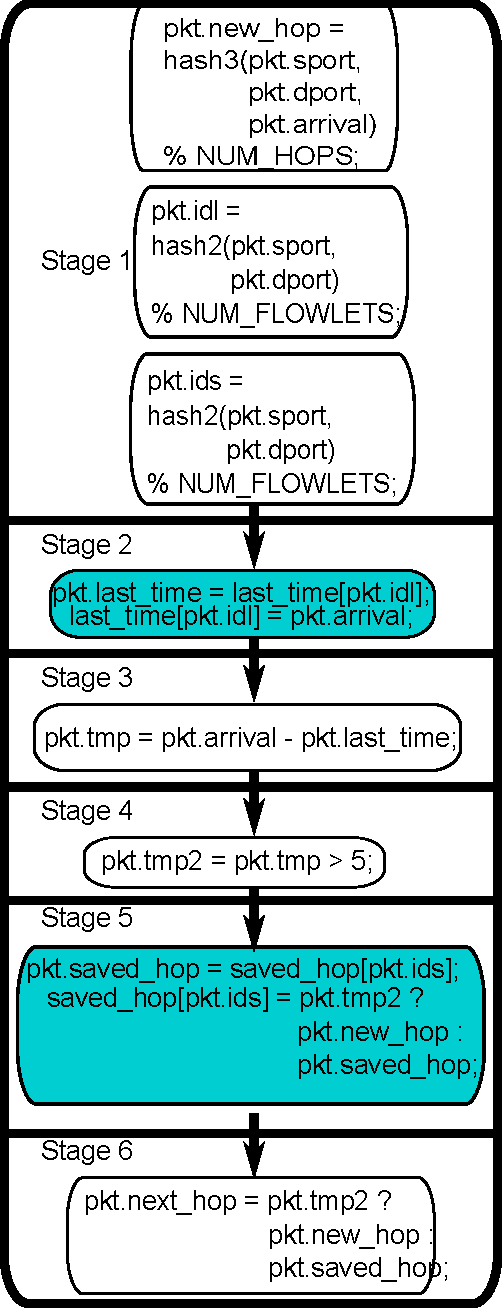
\includegraphics[width=0.8\columnwidth]{pipe.pdf}
\caption{Compiled 6-stage \absmachine pipeline implementing flowlet
switching.  Control flows from top to bottom. Atoms manipulating state are
shaded in blue.}
\label{fig:flowlet_pipeline}
\end{minipage}
\end{figure*}

To program a data-plane algorithm, a programmer would write code in
\pktlanguage using packet transactions (Figure~\ref{flowlet_code}) and then use
the \pktlanguage compiler to compile to an atom pipeline for a \absmachine
machine (Figure~\ref{fig:flowlet_pipeline}). We first describe packet
transactions in greater detail by walking through an example
(\S\ref{ss:flowlet}). Next, we discuss constraints in \pktlanguage
(\S\ref{ss:constraints}) informed by the domain of line-rate switches. We then
discuss how packet transactions are triggered (\S\ref{ss:guards}) and how
multiple transactions are handled (\S\ref{ss:multiple}).

\subsection{\pktlanguage by example}
\label{ss:flowlet}

We now illustrate programming using packet transactions in \pktlanguage, using
flowlet switching~\cite{flowlets} as an example. Flowlet switching is a
load-balancing algorithm that sends bursts of packets (called flowlets) from a
TCP flow on different paths, provided the bursts are separated by a large
enough time interval to ensure packets do not arrive out of order at a TCP
receiver. Figure~\ref{fig:flowlet_code} shows flowlet switching in
\pktlanguage. For simplicity, we hash only the source and destination ports; it
is easy to extend it to the full 5-tuple.

This example demonstrates the core language constructs in \pktlanguage. All
packet processing happens in the context of a packet transaction (the function
\texttt{flowlet} starting at line 17). The function's argument {\tt pkt}
declares the fields in a packet (lines 5--12)\footnote{We use fields to refer
to both packet headers such as source port ({\tt sport}) and destination port
({\tt dport}) and packet metadata ({\tt id}).} that can be referenced by the
function body (lines 18--32).  The function body can also modify persistent
switch state using global variables (e.g.  \texttt{last\_time} and
\texttt{saved\_hop} on lines 14 and 15, respectively).

Conceptually, the switch invokes the packet transaction function on each
incoming packet sequentially. To the programmer, the function modifies the
passed-in packet argument and runs to completion before processing the next
packet.  The function may invoke \textit{intrinsics} such as \texttt{hash2} on
line 23 to use hardware accelerators such as hash generators.  The \pktlanguage
compiler uses an intrinsic's signature to infer dependencies and supplies a
canned run-time implementation, but otherwise does not analyze an intrinsics's
internal behavior. When compiled to a \absmachine machine
(\S\ref{s:absmachine}), the \pktlanguage compiler (\S\ref{s:compiler}) converts
the code in Figure~\ref{fig:flowlet_code} into the atom pipeline in
Figure~\ref{fig:flowlet_pipeline}.

\subsection{Constraints on the language}
\label{ss:constraints}

The overall language is a constrained subset of C
(Table~\ref{tab:restrict}).  These constraints are required for
deterministic performance.  Memory allocation, unbounded iteration
counts, and unstructured control flow all cause variable performance,
which may prevent an algorithm from achieving line rate.
Furthermore, all accesses to a given array within one execution of a
transaction, i.e. one packet, must use the same array index. For
example, all read and write accesses to the array \texttt{last\_time}
use the index \texttt{pkt.id}, which is constant for each packet, but
can change between packets. This restriction mirrors restrictions on
memories, where supporting distinct read and write addresses every
clock cycle is challenging.
%TODO: Try and address this.
%\MA{Do we model this restriction in PISA?
%  It would be better to add it to Sec 2.}

\begin{table}
  \begin{tabular}{p{0.9\columnwidth}}
    No iteration (while, for, do-while).\\
    No goto, break, or continue.\\
    No pointers.\\
    No dynamic memory allocation / heap.\\
    Array index is constant for each transaction execution.\\
    No access to data i.e. unparsed portion of the packet.\\
    No arrays in packet fields.\\
  \end{tabular}
  \caption{Restrictions in \pktlanguage}
  \label{tab:restrict}
\end{table}

\subsection{Triggering packet transactions}
\label{ss:guards}
Packet transactions specify \textit{how} to process packet headers and/or
state.  To specify {\em when} to run packet transactions, we provide a {\em
guard}: a predicate on packet fields that triggers the transaction whenever a
packet matches the guard. An example guard would execute heavy-hitter detection
on all packets arriving on a specific port. The guard can be implemented using
the match key in a match-action pipeline, with the actions being the atoms
resulting from compiling packet transactions to a pipeline of atoms. Because
guards can be easily integrated into a standard match-action pipeline, this
paper only focuses on packet transactions.

\subsection{Handling multiple transactions}
\label{ss:multiple}
So far, we have discussed a single packet transaction. In practice, a switch
would run multiple data-plane algorithms each processing its own subset of
packets. To accommodate multiple transactions, we envision providing a policy
language that specifies pairs of guards and transactions. Realizing a policy is
straightforward when all guards are disjoint. When guards overlap, mutliple
transactions may need to execute on the same subset of packets, requiring a
mechanism to compose two transactions. One approach is to concatenate the two
transaction bodies in an order specified by the user, providing the illusion of
a larger transaction that combines two transactions. We leave a detailed
exploration of these approaches to future work. For the rest of this paper, we
focus only on compiling a single packet transaction.

%\section{A high-level language for data-plane algorithms}
\label{s:language}
%% A closer inspection of these
%%algorithms shows us that the algorithms are characterized by two distinguishing
%%features: a reliance on persistant state and an irregular control flow, both of
%%which make them challenging to implement in hardware and hence in P4 given its
%%low-level nature.
%%
%%As previously described, data-plane algorithms are characterized by an
%%irregular control flow and extensive use of stateful processing. Based on these
%%observations, this section proposes a language to express these algorithms.
%% Alvin: Can you take a stab at easing into this section better.

In this section we describe \pktlanguage, our language for expressing 
data-plane algorithms. The design of \pktlanguage is based on two principles:

\paragraph{A packet-oriented abstraction} 
Each \pktlanguage program is structured using
{\em packet functions}, where each function takes in a single packet
and a set of variables representing the state of the switch as input.
This design is based on the observation that many data-plane algorithms can
be expressed as ones that process each packet individually given the current 
state of the switch. Examples include XXX, and XXX. \ac{are packet functions
supposed to return anything? or do they modify the packet in place? how to 
express things like dropping the input packet?}
We believe this abstraction allows network operators to easily structure
and reason about their algorithms.

\paragraph{Transaction-based semantics} 
To avoid network operators from the need to reason about different execution
paradigms, each statement in \pktlanguage is executed sequentially.
Furthermore, each \pktlanguage packet function is intended to be executed
as a single transaction without any interruption. We adopted this design
from the widespread use of transactions 
in packet processing for software-router platforms. For instance,
Click's Element abstraction~\cite{click} specifies packet processing as
a method invocation that isn't pre-empted.  The Linux qdisc
subsystem~\cite{qdisc} exposes an enqueue and dequeue method that specific
algorithms can implement. Intel's IXP architecture for NPUs uses a construct
resembling transactions called a Packet-Processing Stage
(PPS)~\cite{npu} to express packet processing code.

With that in mind, Figure~\ref{fig:language} shows the grammar of \pktlanguage.
As an imperative language, the language constructs are mostly standard.
Notable features include the declaration of stateful variables outside of each
packet function, where such variables represent the state of the switch 
(e.g., XXX, and XXX) that are accessible inside each packet function, and 
modeling of the packet header \ac{check} fields as members of the {\tt Packet} class,
to be defined as part of the program.
The language does not have any looping constructs or memory allocation, 
as they cannot be easily implemented
in network hardware \ac{check if true}. Furthermore,
we currently restrict stateful variables and packet fields to be primitive
values (i.e., no arrays or structures).

\begin{figure}
\begin{small}
\begin{lstlisting}
v $\in$ variables ::=
  <stateful vars> | pkt.f | <constants>
op $\in$ binary ops ::= + | - | * | < | == | ! | && | || 
s $\in$ statements ::= 
  v$_1$ op v$_2$; | if (v$_1$) { s$_1$; } else { s$_2$; } | s$_1$ ; s$_2$ 
f $\in$ packet function ::= 
  <function name>(Packet pkt) { s }
p $\in$ program ::=
  <stateful vars decl> <packet fields decl> f
\end{lstlisting}
\end{small}
\label{fig:language}
\caption{\pktlanguage grammar}
\end{figure}


As an example, \ref{fig:flow}(a) \ac{can you add labels to the figure} shows
the body of a packet function written using 6 lines of \pktlanguage code
that implements load balancing using flowlet
switching~\cite{flowlets}.


% old text below
\if 0

To motivate a language for these algorithms, we first observe that most, if not all
data-plane algorithm can be expressed as a function that takes in a single
packet and a set of persistent state variables as input. This function then
runs to completion without interruption, modifying the packet and the
persistent state variables in the process. Further, conceptually, only one
packet is processed by this function at any given instant.

This view of data-plane algorithms suggests a natural way to structure them: as
transactions where a function specifies all the required state manipulation and
control flow required for packet processing. The use of transactions is
widespread in packet processing for software-router platforms. For instance,
Click's Element abstraction~\cite{click} specifies packet processing as
a method invocation that isn't pre-empted.  The Linux qdisc
subsystem~\cite{qdisc} exposes an enqueue and dequeue method that specific
algorithms can implement. Intel's IXP architecture for NPUs uses a construct
resembling transactions called a Packet-Processing Stage
(PPS)~\cite{npu} to express packet processing code.
% https://github.com/torvalds/linux/blob/master/net/sched/sch_codel.c#L256

Relative to these prior systems, our contribution is in observing that
transactions can be profitably used to express data-plane algorithms for
high-speed line-rate switches as well. Realizing this practically requires us
to design a language that expresses packet processing within the body of the
transaction. A good language would strike the right balance between ease of
expression and ease of implementation. Programmable hardware switches
---although a significant advance over their fixed-function counterparts---are
still very restricted in the processing that they do on every packet. This
restriction is required to remain competitive with fixed-function switches.

Based on these observations, we describe our language for packet processing
(Figure~\ref{fig:language}). Our language is a heavily constrained subset of C
that removes all iterative constructs (while, do-while, for, break, continue),
arrays, heaps, and memory allocation. State variables are represented as global
variables. We permit structures to represent packet processing alone, and immediately
desugar these to scalar variables (\S\ref{s:compiler}).

Forbidding loops and other sources of variable performance like memory
allocation, and array scans allows the user to only express code whose
execution latency can be bounded at compile time.  While this may seem overly
restrictive, this is required for the underlying architecture
(\S\ref{s:architecture}), which has deterministic performance regardless of the
traffic pattern or program being run.

\fi

%% Anirudh: Not sure if the text below makes sense/fits.
%% This results in a different set of
%% tradeoffs than what programmers are typically used to: a larger program does
%% not take longer to run. Instead, it may not run at all or might need to be
%% approximated until it can run (\S\ref{ss:approximation}).

\section{The \pktlanguage compiler frontend}

We now describe the \pktlanguage compiler frontend. The compiler frontend
operates only on sequential code blocks, allowing us to borrow well-established
techniques from the compiler literature~\cite{muchnik}. However, as we show
throughout this section, constraining \pktlanguage allows us to considerably
simplify the compiler relative to mainstream compilers.

\subsection{Lexical, syntactic, and semantic analysis}
\pktlanguage's syntax is a subset of C, implying that all \pktlanguage are
well-formed C programs that can be compiled by a C compiler like
clang~\cite{clang}. We use clang's library interface~\cite{libclang} to
generate an Abstract Syntax Tree (AST) for a packet transaction written in
\pktlanguage. The remaining compiler passes all operate on an AST produced by
clang.

Embedding \pktlanguage within C has several benefits. It allows to reuse
clang's industrial strength frontend and catches several compiler errors with
no additional effort.  It also allows us to use C's macro preprocessor for
constants. Finally, opaque functions representing hardware primitives (e.g.
hashes and checksum), can be implemented using arbitrary C code and linked with
\pktlanguage code before running the resulting binary on our abstract machine.

\subsection{Converting to straight-line code}
A packet transaction's body can contain convoluted control flow using if-else
statements. Control flow complicates dependence analysis. We eliminate control
flow by transforming if-else statements using the C conditional operator,
starting from the innermost if statements and recursing outwards
(Figure~\ref{fig:if_convert}). This is similar to if
conversion~\cite{allen_if_conversion}, but is much simpler because only the if
and else constructs alter control flow in \pktlanguage and all other forms of
control transfers (break, continue, loops) are forbidden.

We illustrate this on a code fragment from Figure~\ref{fig:flowlet} below:
\begin{figure}
\begin{tiny}
\begin{lstlisting}
if (pkt.arrival_time - last_time[pkt.id1] > FLOWLET_THRESHOLD) {
  saved_hop[pkt.id0] = pkt.new_hop;
}
\end{lstlisting}
\end{tiny}
\begin{center}
is transformed into
\end{center}
\begin{tiny}
\begin{lstlisting}
pkt.tmp0 = pkt.arrival_time - last_time[pkt.id1] > FLOWLET_THRESHOLD;
saved_hop[pkt.id0] = pkt.tmp0 ? pkt.new_hop : saved_hop[pkt.id0];
\end{lstlisting}
\end{tiny}
\caption{Conversion to straight-line code}
\label{fig:if_convert}
\end{figure}

This transformation creates straight-line code, where control always passes
from one statement to the next without any branching. Straight-line code
considerably simplifies the rest of the compiler.

\subsection{Identifying state variables}

We next identify all state variables used in a packet transaction, both arrays
and scalars. State variables represent persistent state stored on the switch
that modifies the behavior of the packet transaction from one step to the next.
In Figure~\ref{fig:flowlet}, \texttt{last\_time} and \texttt{saved\_hop} are
both array-based state variables.

%%We handle state variables differently from packet variables for two reasons.
%%All operations on a particular state variable must happen within one
%%\absmachine atom. This reflects the reality that sharing state variables across
%%atoms or stages is technically challenging because it would require
%%multi-ported memories. Further, all state updates on a state variable should be
%%completed before the next packet is processed. Otherwise, the next packet could
%%see stale values, which would violate the transactional specification.

To identify state variables, we scan the straight-line AST produced by the
previous pass, looking for scalar variables or arrays. For each state variable,
we create a \textit{read flank} to read the state variable into a packet
temporary (if it's an array, we move the indexing expression into the prologue
as well), replace all occurences of the state variable with the packet
temporary, and create a \textit{write flank} that writes the packet temporary into the
state variable.  Figure ~\ref{fig:stateful_flanks} shows this transformation on
the function body of the flowlet switching example.

\begin{figure}
\begin{tiny}
\begin{lstlisting}
pkt.new_hop = hash3(pkt.sport, pkt.dport, pkt.arrival_time \% 64;
pkt.id1 = hash2(pkt.sport, pkt.dport) \% 8000;
pkt.id0 = hash2(pkt.sport, pkt.dport) \% 8000;
pkt.tmp0 = pkt.arrival_time - last_time[pkt.id1] > 5;
saved_hop[pkt.id0] = pkt.tmp0 ? pkt.new_hop : saved_hop[pkt.id0];
last_time[pkt.id1] = pkt.arrival_time;
pkt.next_hop = saved_hop[pkt.id0];
\end{lstlisting}
\end{tiny}
\begin{center}
is transformed into
\end{center}
\begin{tiny}
\begin{lstlisting}
// Read prologue for saved_hop and last_time
pkt.id0 = hash2(pkt.sport, pkt.dport) \% 8000;
pkt.saved_hop0 = saved_hop[pkt.id0];
pkt.id1 = hash2(pkt.sport, pkt.dport) \% 8000;
pkt.last_time0 = last_time[pkt.id1];

pkt.new_hop = hash3(pkt.sport, pkt.dport, pkt.arrival_time) \% 64;
pkt.tmp0 = pkt.arrival_time - pkt.last_time0 > 5;
pkt.saved_hop0 = pkt.tmp0 ? pkt.new_hop : pkt.saved_hop0;
pkt.last_time0 = pkt.arrival_time;
pkt.next_hop = pkt.saved_hop0;

// Write epilogue for saved_hop and last_time
saved_hop[pkt.id0] = pkt.saved_hop0;
last_time[pkt.id1] = pkt.last_time0;
\end{lstlisting}
\end{tiny}
\caption{Adding read and write flanks for state variables}
\label{fig:stateful_flanks}
\end{figure}

At the end of this pass, the code resembles assembly code for a load-store
architecture: state variables are only accessed through reads and writes, and
all arithemtic operations happens on packet variables. Restricting the set of
operations on state variables allows us to simplify reasoning about state
variables when we compile \pktlanguage to the abstract machine
(\S\ref{s:machine}).

% TODO: Mention how resticting accesses to arrays using read/write addresses
% allows us to simplify the stateful pass.

% Any reason, we should be running SSA after stateful_flanks and not the
% other way around? Run it and see.
% I tried this in jayhawk and things don't work. Here's why.
% Stateful_flanks almost always destroys SSA because if you have something any
% state variable write of the form s = pkt.f; it will be transformed into
% pkt.tmp = s;
% pkt.tmp = pkt.f;
% s = pkt.tmp;
% which already destroys SSA.

\section{A Machine Model for Line-rate Switches}
\label{s:absmachine}
% TODO: Consider renaming to PISA
\begin{figure*}[!t]
  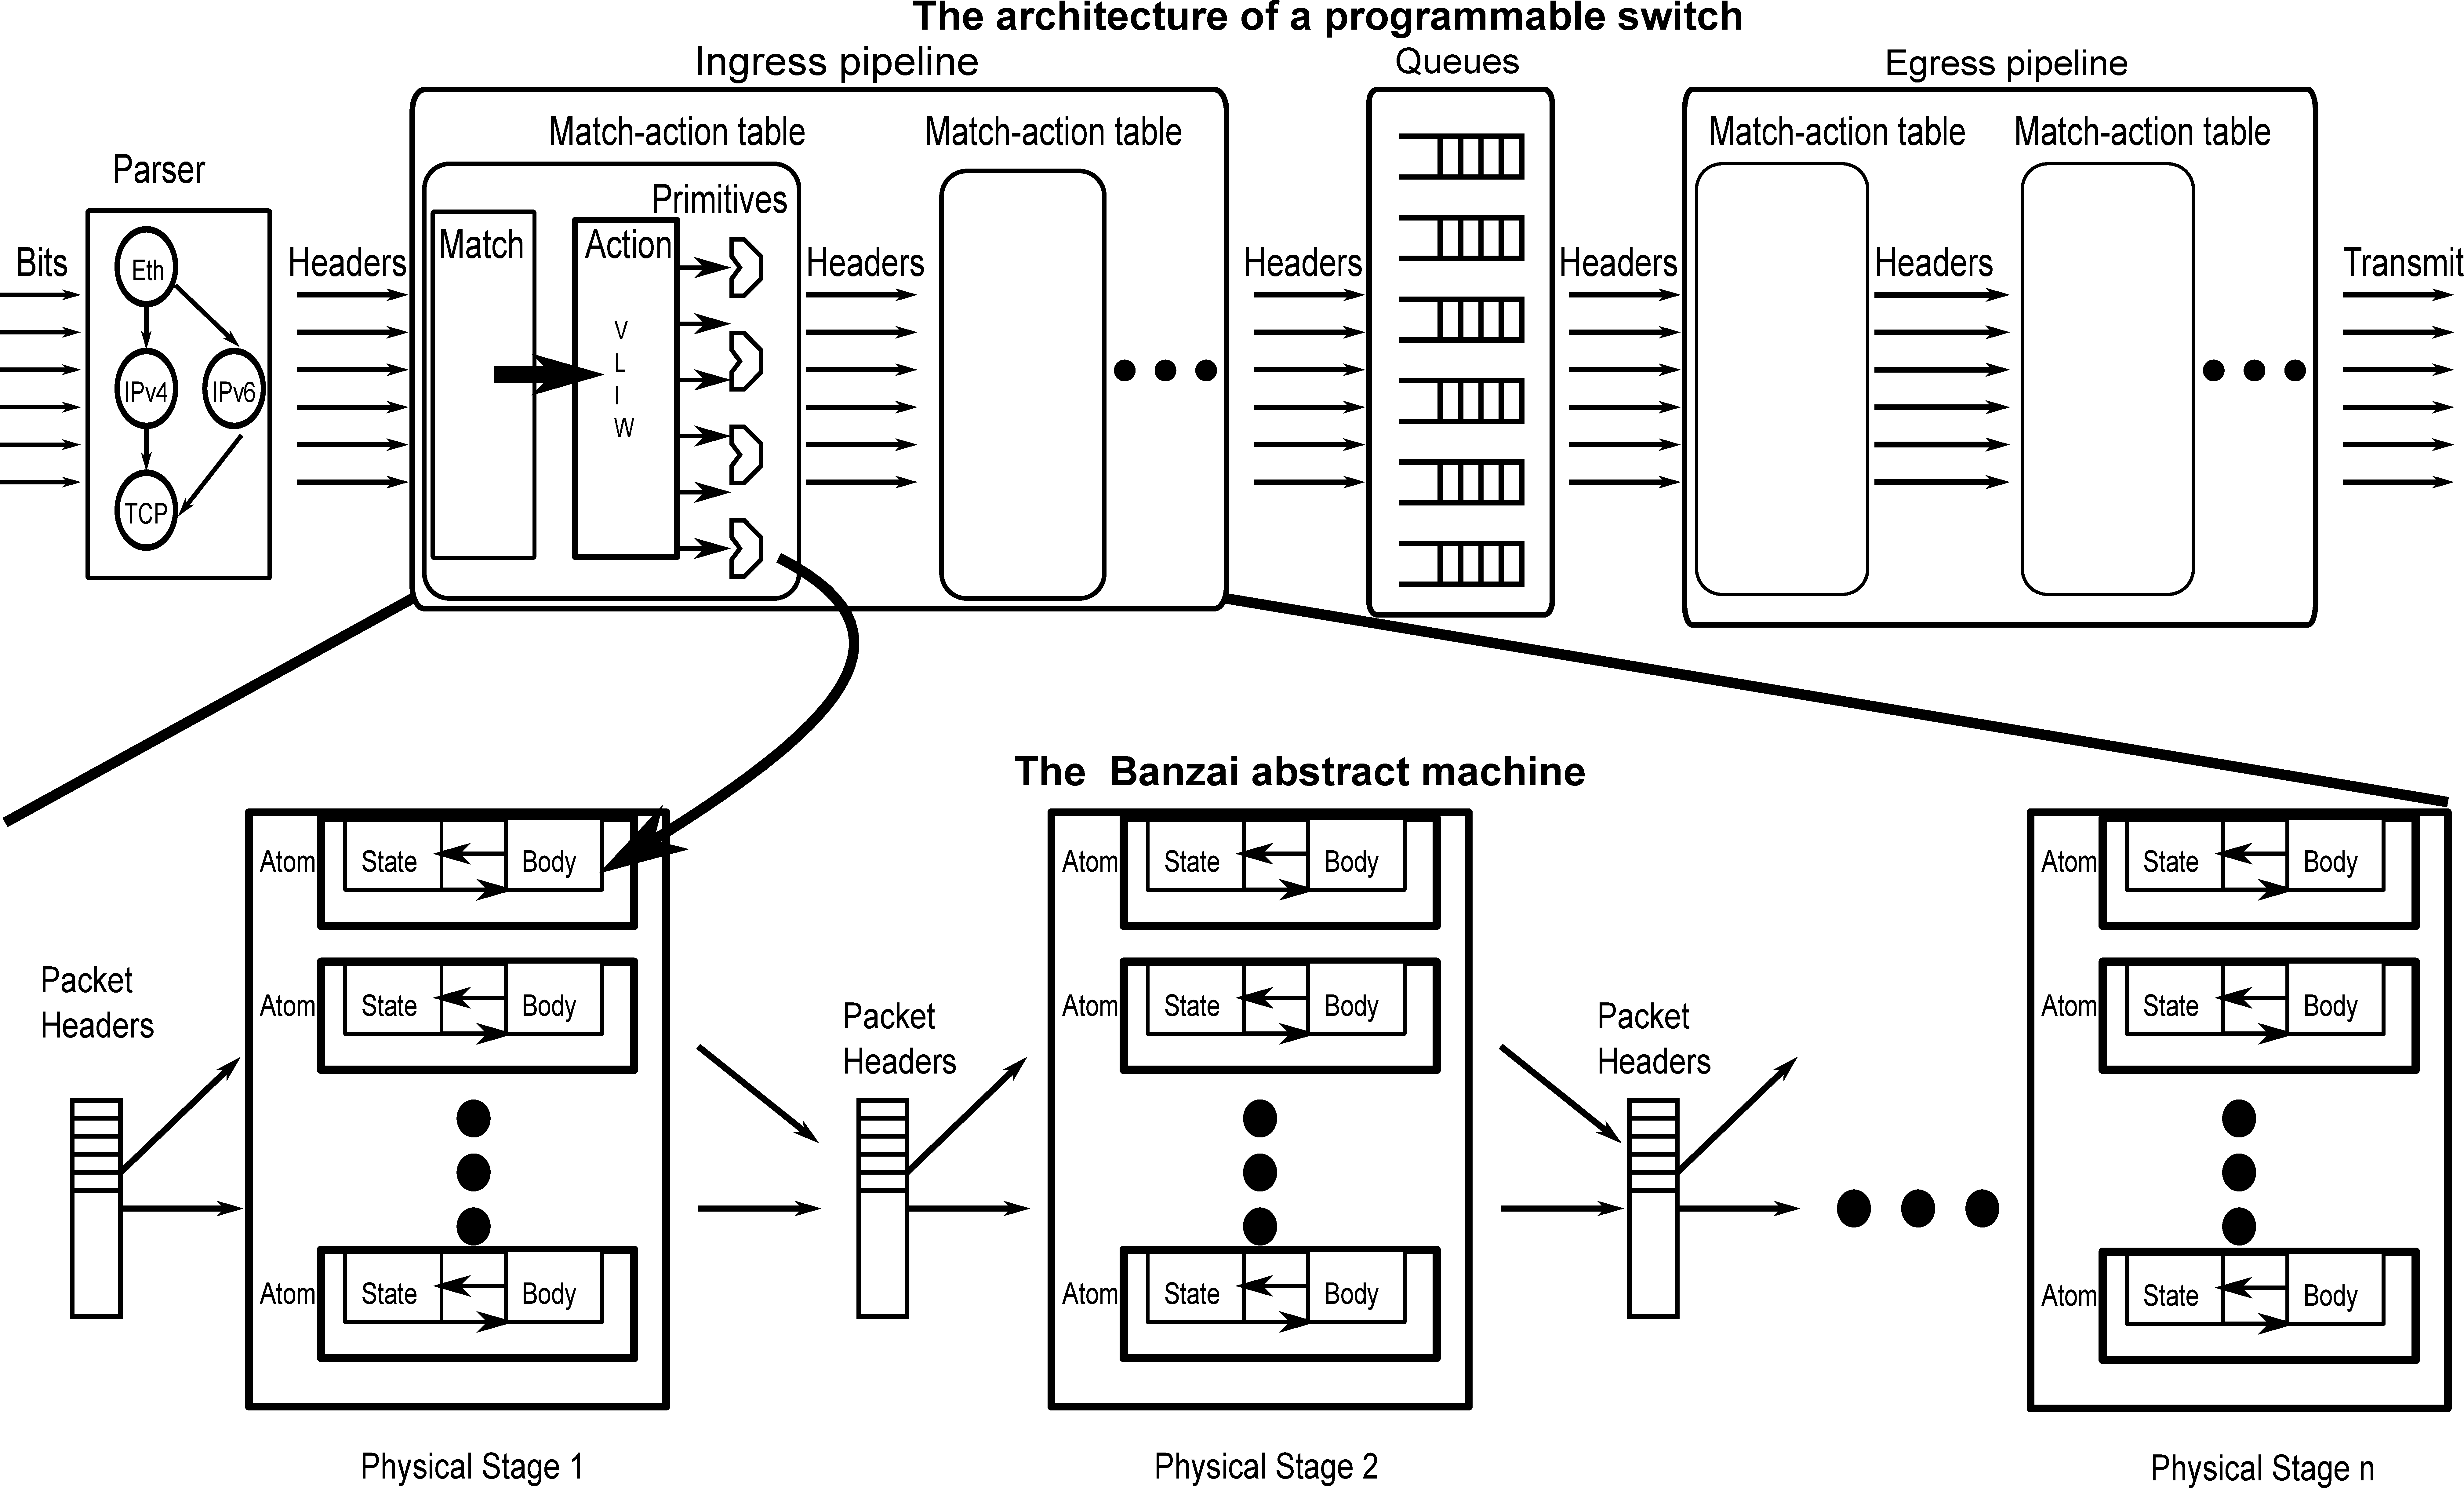
\includegraphics[width=\textwidth]{banzai.pdf}
  \caption{The \absmachine machine model and its relationship to
  programmable switch architectures.}
  \label{fig:switch}
\end{figure*}

\absmachine is a machine model for programmable line-rate switches that serves
as the compiler target for \pktlanguage programs.  \absmachine's design is
inspired by recent programmable switch architectures such as Barefoot's
Tofino~\cite{tofino}, Intel's FlexPipe~\cite{flexpipe}, and Cavium's XPliant
Packet Architecture~\cite{xpliant}. \absmachine abstracts these architectures
and extends them with stateful processing units to implement data-plane
algorithms. These processing units, called {\em atoms}, model the set of
operations that a hardware target can execute at line rate.

\subsection{Background: Programmable switches}
Packets arriving at a programmable switch~(Figure~\ref{fig:switch}) are parsed
by a programmable parser that turns packets into header fields. These header
fields are first processed by an ingress pipeline consisting of match-action
tables arranged in stages. Processing a packet at a stage may modify its header
fields as well as some persistent state at that stage. Each stage has access
only to its own local state. To share state between stages, it must be carried
forward in packet headers. Following the ingress pipeline, the packet is
queued. Once the packet is dequeued by the switch scheduler, it is processed by
a similar egress pipeline before being transmitted.

To reduce chip area, the ingress and egress pipelines are shared across switch
ports.  Each pipeline handles aggregate traffic belonging to all ports on the
switch, at all packet sizes.  For instance, a 64-port switch with a line rate
of 10 Gbits/s per port and a minimum packet size of 64 bytes needs to process
around a billion packets per second~\cite{rmt}.  Equivalently, with a clock
frequency of 1 GHz, each pipeline stage needs to process one packet every clock
cycle (1 ns).  The need to handle one packet per clock cycle is typical because
switches are designed for the highest port count and line rate for a given chip
area. We assume one packet per clock cycle throughout the paper.\footnote{For
concreteness, we assume a 1 GHz clock frequency.}
%TODO: Define line rate.

Having to process a packet every clock cycle in each stage greatly
constrains the operations that can be performed on each packet. In
particular, any packet operation that modifies state visible to the
next packet {\em must} finish execution in a single clock cycle (see
\S\ref{ss:atoms} for details). Because of this restriction,
programmable switching chips provide a small set of processing units
or primitives for manipulating packets and state in a stage, unlike in
software routers. These processing units determine what algorithms can
run on the switch at line rate.

The challenge for us is to develop primitives that allow a broad range of
data-plane algorithms to be implemented, and to build a compiler to map a
user-friendly description of an algorithm to the primitives provided by a
switch.

\subsection{The \absmachine machine model}

\absmachine (the bottom half of Figure~\ref{fig:switch}) models the data-plane
components of an ingress or egress switch pipeline, consisting of a number of
stages executing synchronously on every clock cycle. Each stage processes one
packet every clock cycle (1 ns) and hands it off to the next. \absmachine
models the computation within a match-action table in a stage (i.e., the action
half of the match-action table), but not the match semantics (e.g., direct, or
ternary) (we discuss how to embed these computations in a standard match-action
pipeline in \S\ref{ss:guards}).  \absmachine does not model packet parsing and
assumes that packets arriving to it are already parsed.

\subsection{Atoms: \absmachine's processing units}
\label{ss:atoms}

Each pipeline stage in \absmachine contains a {\em vector of
  atoms}. All atoms in the vector execute in parallel on every clock
cycle.  Informally, an atom is an atomic unit of packet processing
supported natively by a \absmachine machine.
The atoms provided by 
a \absmachine machine form its instruction set.
Atoms may modify persistent state stored on the
switch. In contrast to instruction sets for CPUs, GPUs, DSPs, and
NPUs, the atoms for a \absmachine machine need to be substantially
richer to run real-world data-plane algorithms at line rate. We
explain why with an example.

Suppose we need to atomically increment a state variable stored on the switch
to count packets. One approach would be to have hardware support for three
simple single-cycle operations: \textit{read} some memory in the first clock
cycle, \textit{add} one in the next, and \textit{write} it to memory in the
third. This approach, however, does not provide atomic isolation. To see why,
suppose packet $A$ increments the counter from 0 to 1 by executing the read,
add, and write operations at clock cycles 1, 2, and 3 respectively.  If packet
$B$ issues the read at time 2, it will increment the counter again from 0 to 1,
when it should be 2. Locks over the shared counter are a potential
solution. However, locking causes packet $B$ to wait during packet $A$'s
increment, and the switch no longer sustains line rate of one packet every
clock cycle.\footnote{Wait-free objects~\cite{herlihy_wait} are an alternative
  to locking, but are typically too complex for hardware.} CPUs employ microarchitectural
  techniques such as operand forwarding to address this problem, but these techniques
  suffer from occasional pipeline stalls, which prevents line-rate
  performance from being achieved.
%% TODO: Not mentioning that shared memory is costly. Because, while that's true.
%% there are parts of the switch pipeline that use it (such as the scheduler).

\absmachine provides an atomic increment operation in hardware with an {\em
atom} to read memory, increment it, and write it back in a single stage within
one clock cycle. It uses the same approach to implement other atomic operations
at line rate.

Formally, an atom is a body of sequential code. It may also contain internal
state local to the atom. An atom completes execution of the entire body of
sequential code, modifying a packet and any internal state before processing
the next packet. The designer of a programmable switch would develop these
atoms, and expose them to a switch compiler as the programmable switch's
instruction set.
%%\ac{does this mean we could have invented a new
%%instruction to represent each atom, and the current representation as a
%%body of (C-like?) sequential code is simply convenience for people to 
%%implement different banzai machines?}
%%No. You need someway to represent an atom's functionality to the compiler.
%% like expression trees / tiles for instruction selection.

Using this representation, a switch counter that wraps around at a
value of 100 can be written as the atom:\footnote{We use {\tt p.x} to
  represent field {\tt x} within a packet {\tt p} and {\tt x} to
  represent a state variable {\tt x} that persists across packets.}
\begin{lstlisting}[style=customc, numbers=none, frame=none]
if (counter < 99)
  counter++;
else
  counter = 0;
\end{lstlisting}
Similarly, a stateless operation like setting a packet field
(e.g. P4's {\tt modify\_field} primitive~\cite{p4spec}) can be written
as the atom:
\begin{lstlisting}[style=customc, numbers=none, frame=none]
  p.field = value;
\end{lstlisting}
Table~\ref{tab:templates} provides more examples of atoms.

We note that---unlike stateful atomic operations such as a counter---stateless
atomic operations are easier to support with basic packet-field arithmetic.
Consider, for instance, the operation {\tt pkt.f1 = pkt.f2 + pkt.f3 - pkt.f4}.
This operation does not modify any persistent switch state because it only
reads and writes packet fields. It can be implemented without violating
atomicity by using two atoms: one atom to add fields f2 and f3 in one pipeline
stage (clock cycle), and another to subtract f4 from the result in the next,
without having to provide one large atom that supports the entire operation.

%%\ac{but I thought you are still implement the whole thing as one single atom
%%right? What's the point here}
%% The point is we can implement this as two atoms without violating atomicity.
%% Explained above.

\subsection{Constraining atoms}
\label{s:atomConstraints}

\textbf{Computational limits:} Atoms need to execute atomically from one packet
to the next, implying that any state internal to the atom must be updated
before the next packet arrives. Further, packets may be separated by as little
as one clock cycle. To guarantee atomicity in the worst case, we mandate that
atom bodies finish execution within one clock cycle, and constrain atom bodies
to do so.

We constrain atom bodies by defining {\it atom templates}
(\S\ref{ss:code_gen}).  An atom template is a program that terminates within a
clock cycle and specifies exactly how the atom is executed. One example is an
ALU with a restricted set of primitive operations to choose from
(Figure~\ref{fig:alu_diag}). Atom templates allow us to create and experiment
with \absmachine machines with different atoms. As programmable switches
evolve, we expect that atoms will evolve as well, but constrained by the
clock-cycle requirement~(\S\ref{ss:perfprog}).
%TODO: Consider removing this last sentence or replacing it with how
%transistor scaling could improve how much we pack into these atoms.

\begin{figure}[h]
  \begin{subfigure}{0.4\columnwidth}
  \begin{center}
  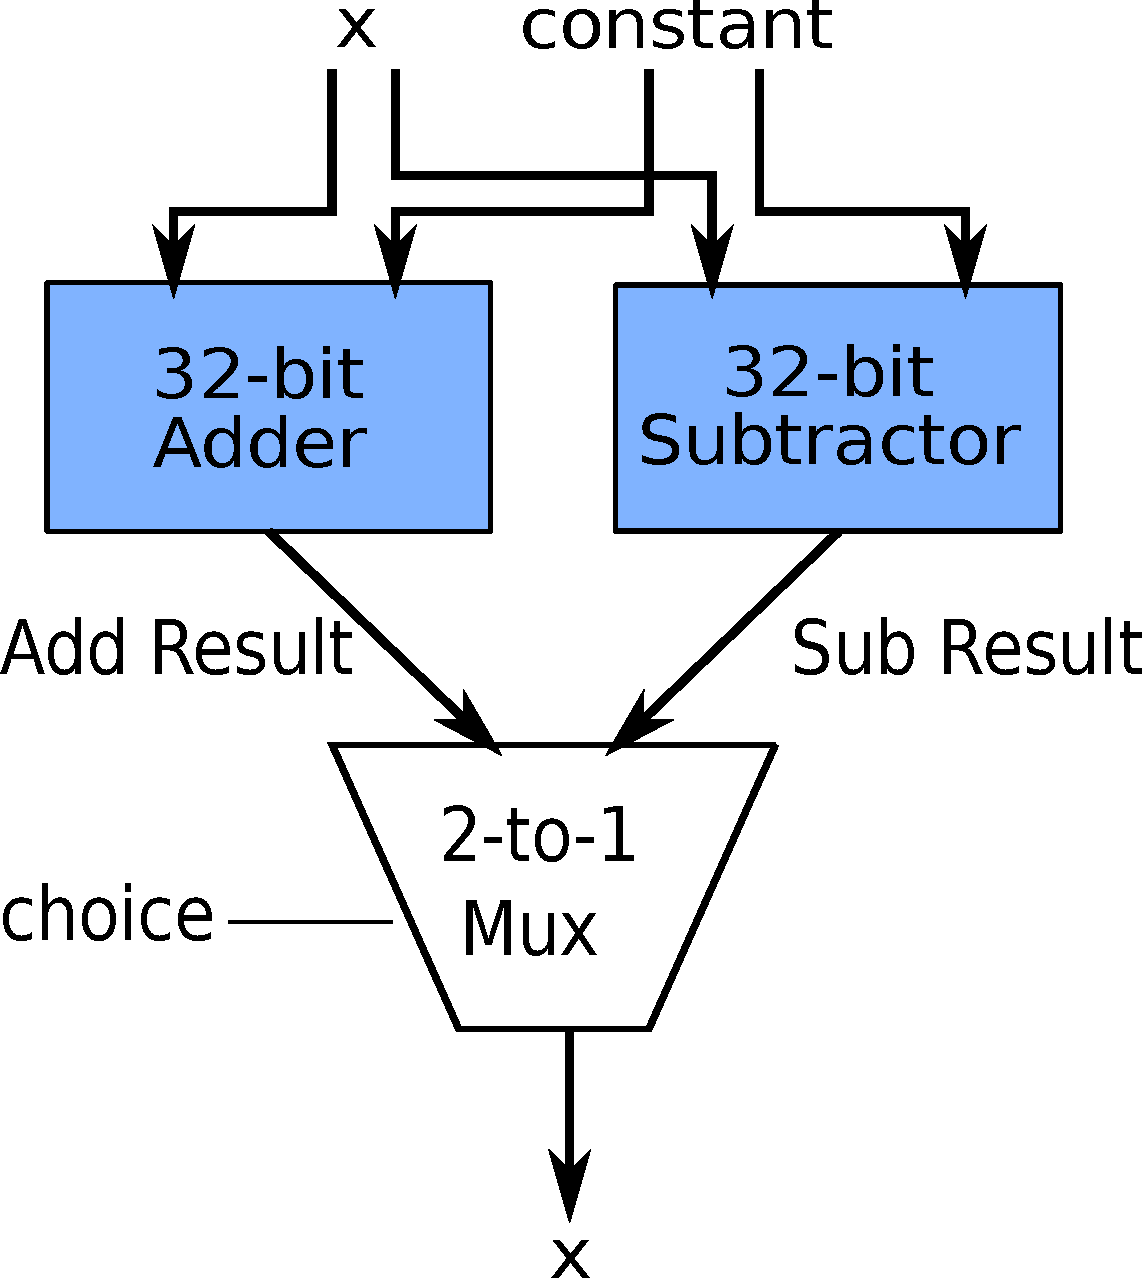
\includegraphics[width=\columnwidth]{circuit.pdf}
  \end{center}
  \caption{Circuit for an atom that can add or subtract a constant from a state variable.}
  \label{fig:alu_diag}
  \end{subfigure}
  \hspace{0.05\columnwidth}
  \begin{subfigure}{0.55\columnwidth}
  \begin{lstlisting}
  bit choice = ??;
  int constant = ??;
  if (choice) {
    x = x + constant;
  } else {
    x = x - constant;
  }
  \end{lstlisting}
  \caption{Circuit representation as an atom template.}
  %Each ``??(n)'' represents a hole that can be filled in with values in $[0, 2^n -1]$.}
  \label{fig:alu_in_sketch}
  \end{subfigure}
  \caption{Atoms and atom templates}
  \label{fig:atom}
\end{figure}

\textbf{Resource limits:} For any real machine, we also need to limit the
number of atoms in each stage (\textit{pipeline width}) and the number of
stages in the pipeline (\textit{pipeline depth}). This is similar to limits on
the number of stages, number of tables per stage, and amount of memory per
stage in programmable switch architectures such as RMT and
FlexPipe~\cite{lavanya_compiler}.

\subsection{What can \absmachine not do?}
\label{ss:limitations}

\absmachine is a good fit for data-plane algorithms that modify a small set of
packet headers and carry out small amounts of stateful or stateless computation
per packet. Data-plane algorithms like deep packet inspection and WAN
optimization require a switch to parse and process the packet payload as
well---effectively parsing a large ``header'' consisting of each byte in the
payload, which is challenging at line rates of 1 GHz. Such algorithms are best
left to general-purpose CPU platforms~\cite{e2}.  Some algorithms require
complex computations, but not on every packet.  For example, consider a
measurement algorithm that periodically scans a large table to perform garbage
collection.  \absmachine's atoms model small computations that occur on every
packet, and are not suitable for operations that span many clock cycles.

% Backend: expr_flattener, instuction_selection, backend synthesis.
% Maybe combine front and middle-end and call clang's semantic + syntactic analysis + type checker, the frontend.
%%
%%%\subsection{Instruction selection}
%%%We next replace portions of the straight-line code with equivalent code that
%%%maps 1:1 to action primitives provided by the underlying hardware. While this
%%%step does require knowledge of the action primitives supported by the
%%%underlying hardware, P4 today already provides action primitives that map
%%%1:1 to those provided by the underlying hardware, allowing us to carry out
%%%instruction selection at the source level itself.
%%%%Anirudh->Alvin: Ok, this is my interpretation of instruction selection
%%%%TODO: Maybe we should just call it action primitive selection?
%%%
%%%As a contrived example, if the underlying hardware supports read and write
%%%operations on stateful memory, but does not support atomic increment operations
%%%on stateful memory, we would have to replace the statement: \texttt{x = x + 1;}
%%%with three statements:
%%%\begin{verbatim}
%%%int tmp1 = x;
%%%int tmp2 = tmp1 + 1;
%%%x = tmp2;
%%%\end{verbatim}
%%%
%%%Other examples of instruction selection include ``flattening''
%%%expressions~\cite{expression_flattening} with deep ASTs into a canonical form
%%%where the right hand side of each assignment is a simple expression that
%%%doesn't contain any expressions within it. These simple expressions would then
%%%map 1:1 to underlying hardware constructs.
%%%
%%%
%%%\subsection{Instruction coalescing}
%%%
%%%As described earlier, RMT is a shared-nothing architecture. State variables
%%%read in a particular stage and updated downstream need recirculation to reflect
%%%the updated value back upstream, creating a vulnerable window of packets that
%%%can read stale state.
%%%
%%%As far as possible, we would like to avoid recirculating packets to emulate
%%%memory sharing across different physical stages. One way to achieve this is to
%%%collapse instructions into the same stage using the greedy partitioning
%%%algorithm outlined in \S\ref{ss:partitioning}. To aid our greedy partitioning
%%%algorithm that only looks at adjacent instructions in deciding whether to
%%%combine instructions into a stage, we first move instructions that access state
%%%variables as close to each other as possible.
%%%
%%%Specifically, if there are two instructions that read or write the same state
%%%variable, we move them as close to each other as possible while respecting
%%%Read-After-Write dependencies. This facilitates combining the instructions in
%%%the greedy partitioning algorithm, which in turn removes the need for
%%%recirculation.
%%%
%%%\subsection{Partitioning based on dependencies}
%%%
%%%At this stage, the code is correct if executed sequentially assuming exactly
%%%one packet ever executes the code. A straightforward partitioning simply
%%%assigns each instruction to a separate stage, but is wasteful. Many
%%%instructions may have no dependencies between them and can be executed in
%%%parallel.
%%%
%%%% TODO: Anirudh->Alvin: Does this read ok?
%%%To determine a better partitioning, we start by assigning each instruction to
%%%its own stage. We then proceed sequentially from the first stage and grow each
%%%stage greedily downward by merging it with the next instruction if possible.
%%%Because instructions in a stage execute in parallel, we use the following
%%%criterion to decide if we can execute instructions in parallel.
%%%\begin{enumerate}
%%%\item If there are no Read-After-Write or Write-After-Write dependencies
%%%between a pair of instructions, it is safe to combine them.
%%%\item If there are only Write-After-Read dependencies between instructions, we
%%%can still combine them because the underlying hardware executes actions within
%%%a stage simultaneously, which preserves the right semantics for
%%%Write-After-Read dependencies.
%%%% TODO: Only works if it fits that particular format
%%%% (state, pkt.f) = (Guarded_Arithmetic(pkt.field, state, pkt.field), state) 
%%%
%%%\item If there is a Read-After-Write dependency where a variable is updated in
%%%one instruction and the updated variable needs to written into another
%%%variable, we can still merge these instructions by replicating the same update
%%%operation for both variables and relying on the fact that both operations
%%%execute in parallel.
%%%% TODO: Only works if it fits that other mold:
%%%% (state, pkt.f) = (Guarded_Arithmetic(pkt.field, state, pkt.field), state) 
%%%% Really, the second one is a superset of the first.
%%%\end{enumerate}
%%%With the above criteria, we merge a stage with the next instruction using our
%%%greedy algorithm if the next instruction can be executed in parallel with every
%%%instruction in the current stage. If this criteria isn't satisfied, we create a
%%%new stage using the next instruction and proceed greedily again until we have
%%%covered all instructions.
%%%
%%%

\section{\tester: verifying compilations}
\label{s:jayhawk}
We next describe our testing infrastructure to verify that the compilation is
correct: the externally visible behavior of the packet transaction
(Figure~\ref{fig:flowlet}) is indistinguishable from its pipelined
implementation (Figure~\ref{fig:pipeline}).

We verify correctness by feeding in the same set of test packets to both the
packet transaction and its implementation and comparing the outputs from both
programs on the set of externally visible fields. To create test packets, we
scan the packet transaction and generate the set of all packet fields read from
or written to by the transaction. We then initialize each of these fields by
sampling uniformly from the range of all 32-bit signed integers. In the future,
we plan to allow the user to specify more precise ranges for each packet field
that can be used for more directed testing.

To compare outputs from the packet transaction and its implementation, we track
renames that occur because of the SSA form. We generate a list of renames due
to SSA and compare each output field in the transactional form with the last
rename of the same output field in the implementation.

We then feed the same number of test packets to both the specification and
implementation and compare outputs at the end of the pipeline. This allows to
quickly ``sanity check'' our compilations and was instrumental in uncovering a
few bugs in various compilation passes during development.
%TODO: I am not sure I completely understand how this testing works.

\section{Evaluation}
% TODO: Is there a good technical reason why every \absmachine machine
% should have exactly one large stateful atom as opposed to many small stateful atoms?

% TODO: Show how pipeline width / depth changes
% by adding more complicated atoms? This might be a little more work though.

% TODO: Do we mention how we had to approximate CONGA? Another option is to create
% an appendix with all the algorithms written in domino.
\label{s:eval}

\begin{table}[!t]
  \begin{scriptsize}
  \begin{tabular}{|p{0.1\textwidth}|p{0.35\textwidth}|}
    \hline
    Atom & Description \\
    \hline
    Write & Write packet field/constant into single state variable. \\
    \hline
    ReadAddWrite (RAW) & Add packet field/constant to state variable (OR) Write packet field/constant into state variable. \\
    \hline
    Predicated ReadAddWrite (RAW) & Execute RAW on state variable only if a predicate is true, else leave unchanged. \\
    \hline
    IfElse ReadAddWrite (IfElseRAW) & Execute two separate RAWs: one each for when a predicate is true or false.\\
    \hline
    Subtract (Sub) & Same as IfElseRAW, but also allow subtracting a packet field/constant. \\
    \hline
    Nested Ifs (Nested) & Same as Sub, but with an additional level of nesting that provides 4-way predication. \\
    \hline
    Paired updates (Pairs) & Same as Nested, but allow updates to a pair of state variables, where predicates can use both state variables. \\
    \hline
  \end{tabular}
  \end{scriptsize}
  \caption{Atoms used in evaluation. Appendix A provides the SKETCH code and
  circuit diagrams for these atoms.}
  \label{tab:templates}
\end{table}

\begin{table}[!t]
  \begin{scriptsize}
    \begin{tabular}{|p{0.08\textwidth}|p{0.3\textwidth}|p{0.03\textwidth}|}
  \hline
  Atom & Circuit & Circuit depth \\
  \hline
  Write & 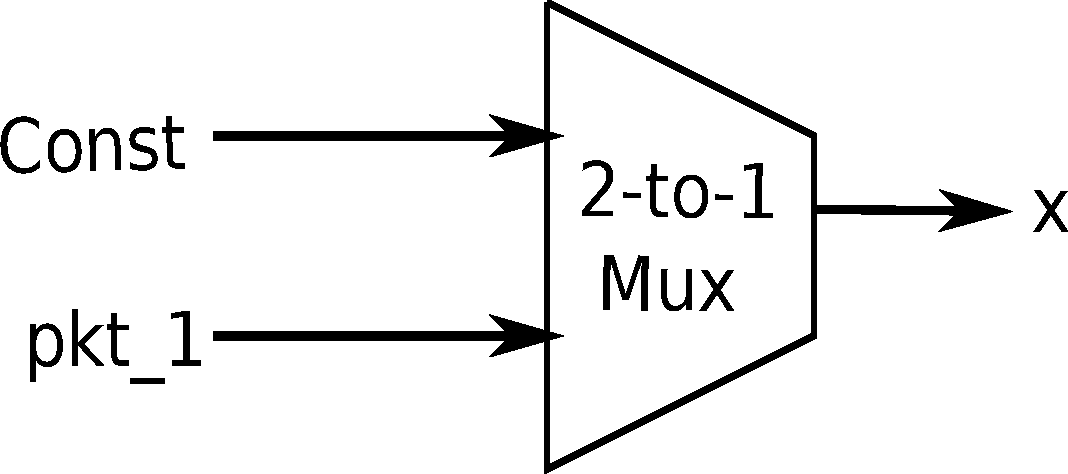
\includegraphics[width=0.2\textwidth]{rw.pdf} & 1 \\
  \hline
  ReadAddWrite (RAW) & 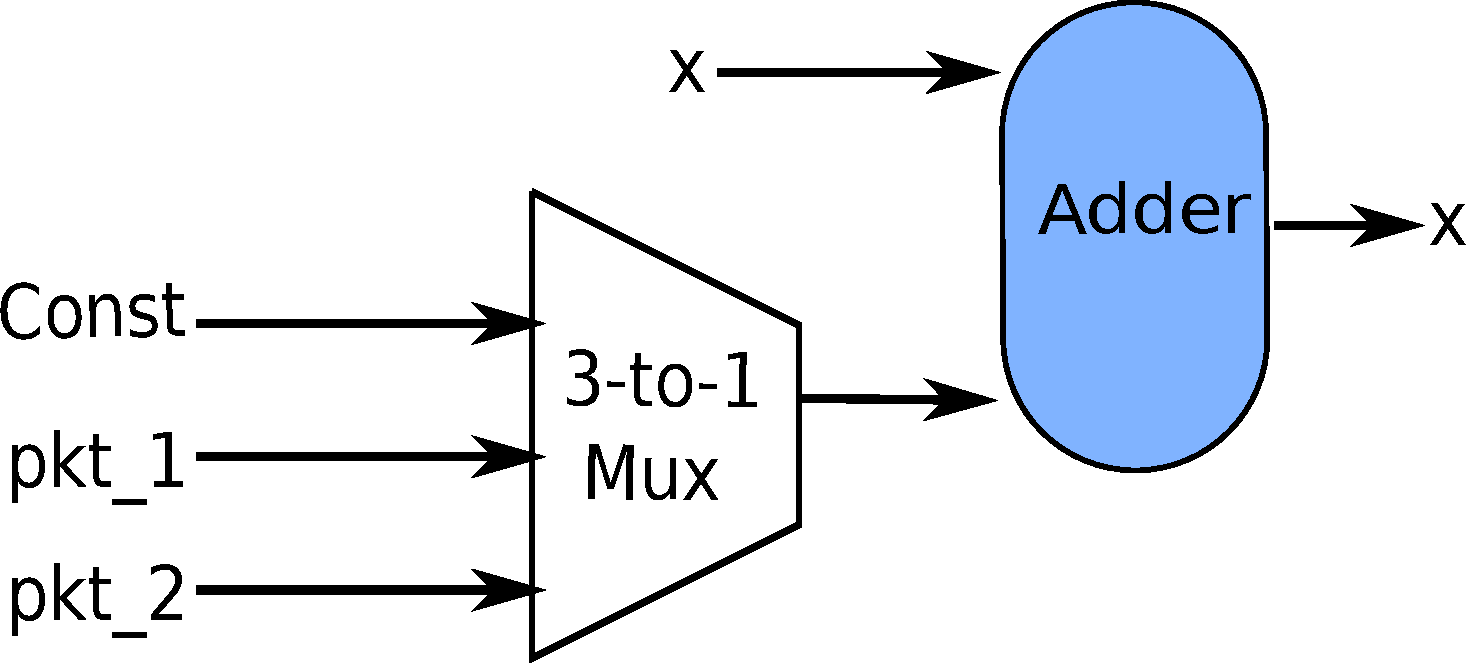
\includegraphics[width=0.2\textwidth]{raw.pdf} & 2\\
  \hline
  \pbox{0.1\textwidth}
  {Predicated\\
  ReadAddWrite (PRAW)} & 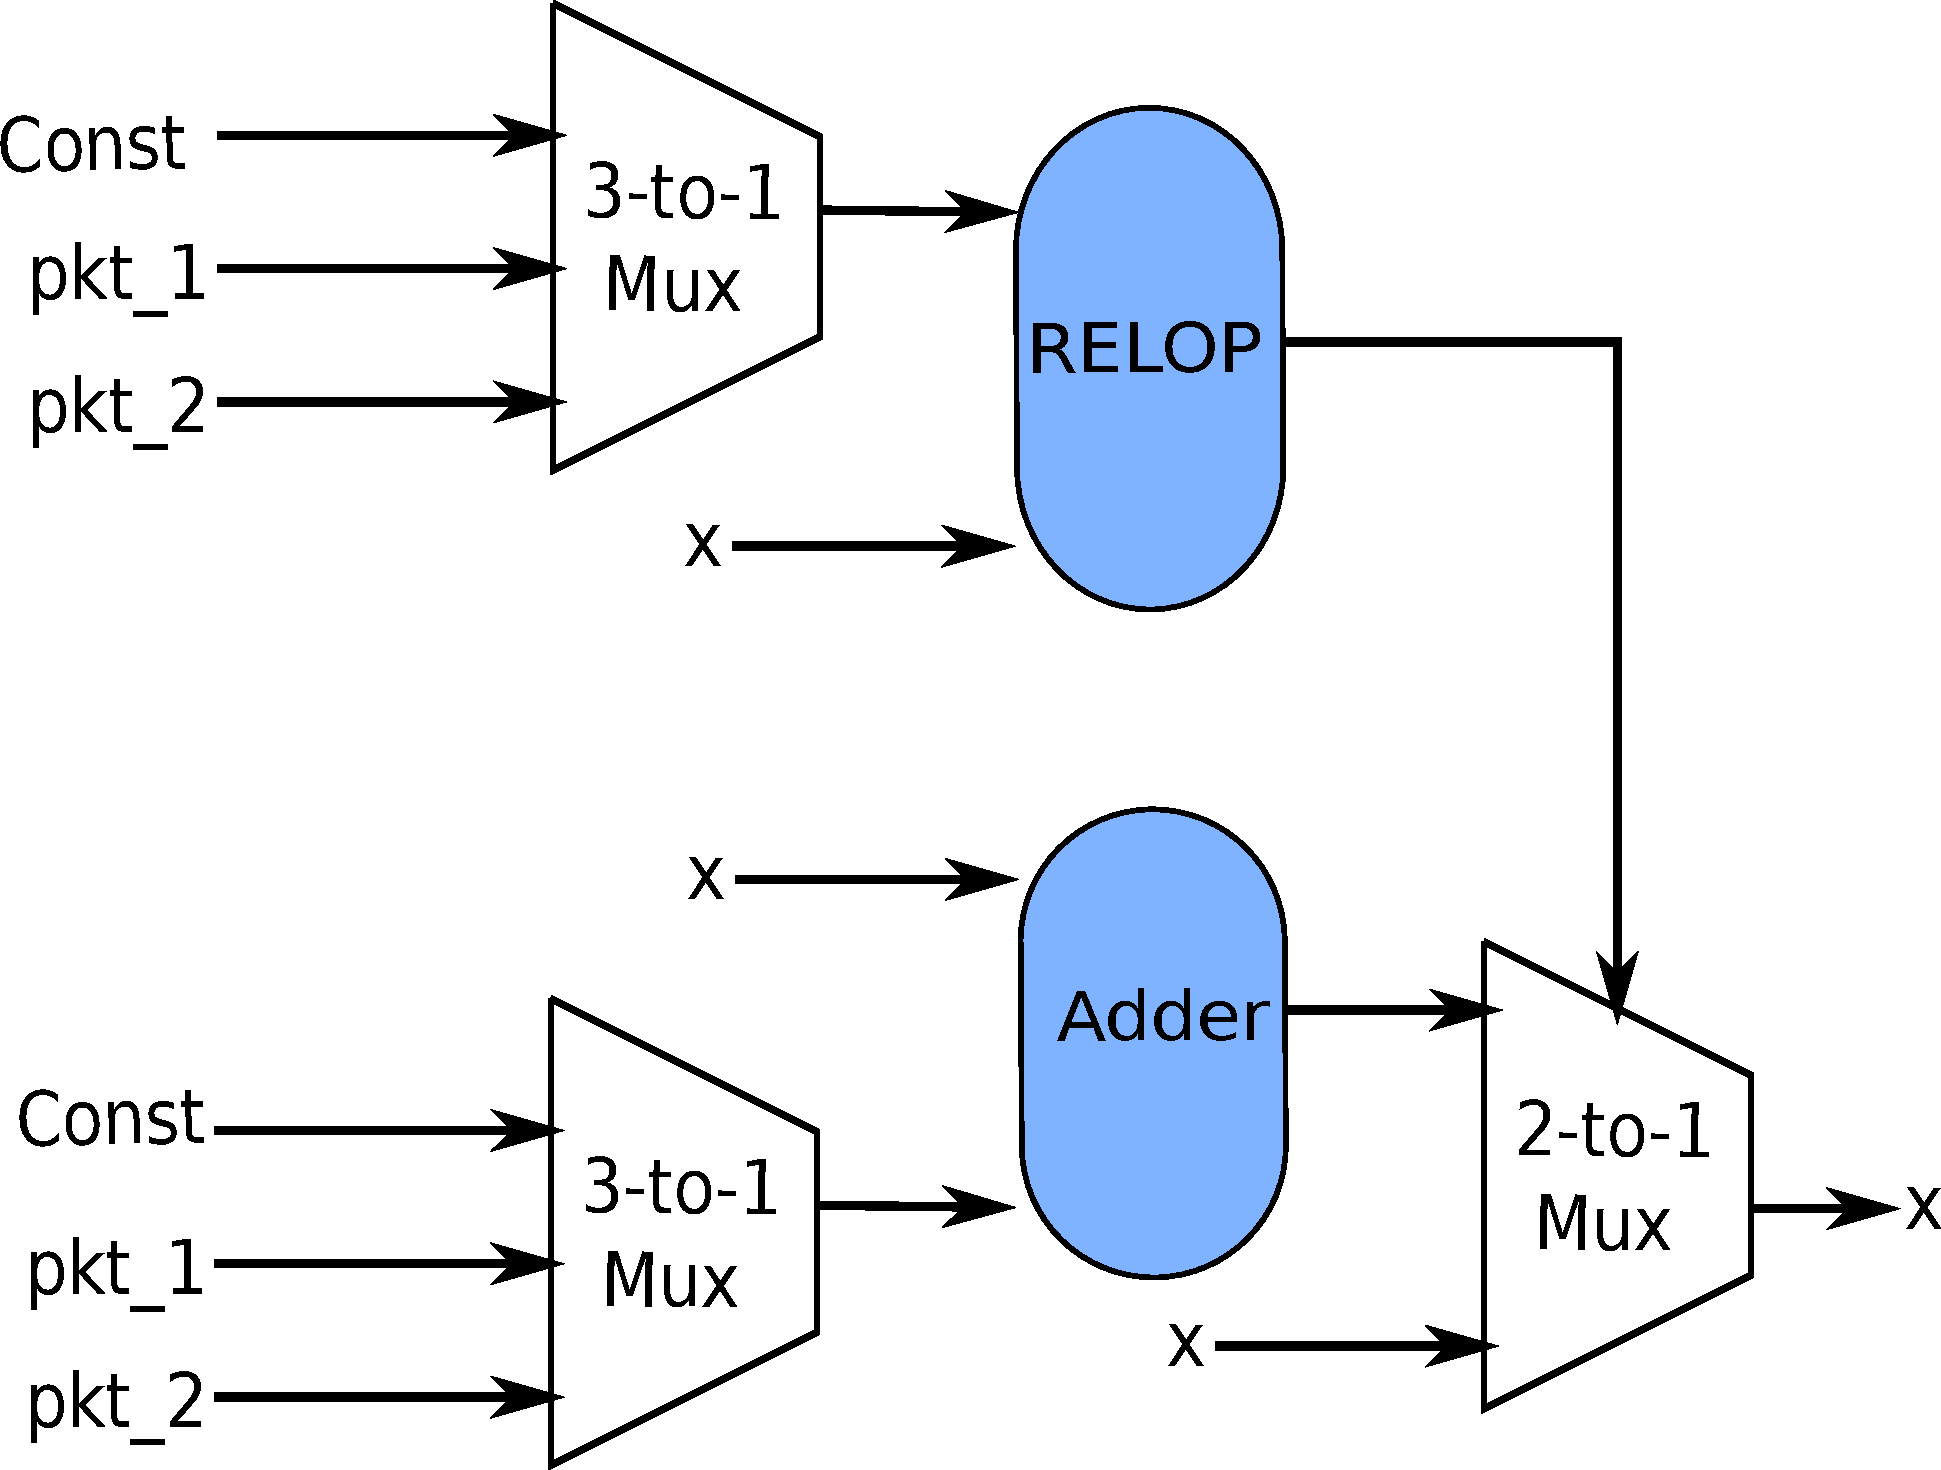
\includegraphics[width=0.3\textwidth]{pred_raw.pdf}  & 3\\
  \hline
  \end{tabular}
\end{scriptsize}
\caption{Circuit depth and propagation delay increases with complexity of atoms.}
  \label{fig:circuit_depth}
\end{table}

\begin{table*}[!t]
  \begin{tabular}{|p{0.16\textwidth}|p{0.47\textwidth}|p{0.09\textwidth}|p{0.06\textwidth}|p{0.07\textwidth}|}
\hline
Algorithm & Stateful computation & Least expressive atom & Pipeline depth, width & Ingress or Egress Pipeline?\\
\hline
\pbox{0.16\textwidth}{Bloom filter~\cite{bloom}\\(3 hash functions)} & \pbox{0.54\textwidth}{Set membership bit on every packet.} & Write & 4, 3 & Either \\
\hline
\pbox{0.16\textwidth}{Heavy Hitters~\cite{opensketch}\\(3 hash functions)} & Increment Count-Min Sketch~\cite{cormode} on every packet. & RAW & 10, 9 & Either \\
\hline
Flowlets~\cite{flowlets} & Update saved next hop if flowlet threshold is exceeded. & PRAW & 6, 2 & Ingress \\
\hline
RCP~\cite{rcp} & \pbox{0.47\textwidth}{Accumulate RTT sum if\\RTT is under maximum allowable RTT.} & PRAW & 3, 3 & Egress \\
\hline
\pbox{0.16\textwidth}{Sampled\\NetFlow~\cite{sampled_nflow}} & \pbox{0.47\textwidth}{Sample a packet if packet count reaches N;\\Reset count to 0 when it reaches N.} & IfElseRAW & 4, 2 & Either\\
\hline
HULL~\cite{hull} & Update counter for virtual queue. & Sub & 7, 1 & Egress \\
\hline
\pbox{0.16\textwidth}{Adaptive\\Virtual Queue~\cite{avq}} & Update virtual queue size and virtual capacity & Nested & 7, 3 & Ingress \\
\hline
CONGA~\cite{conga} & \pbox{0.54\textwidth}{Update best path's utilization/id if we see a better path.\\
                                           Update best path utilization alone if it changes.}  & Pairs & 4, 2 & Ingress\\
\hline
trTCM~\cite{trTCM} & Update token counts for each token bucket & Doesn't map & 7, 3 & Either \\
\hline
CoDel~\cite{codel} & \pbox{0.54\textwidth}{Update:\\Whether we are marking or not.\\Time for next mark.\\Number of marks so far.\\Time at which min. queuing delay will exceed target.}& Doesn't map & 15, 3 & Egress \\
\hline
\end{tabular}
\caption{Data-plane algorithms}
\label{tab:algos}
\end{table*}

To evaluate \pktlanguage, we express several data-plane algorithms
(Table~\ref{tab:algos}) using \pktlanguage and determine if they are
implementable on different \absmachine machines that provide different stateful
atoms (Table~\ref{tab:templates}). Appendix A contains circuit diagrams and
SKETCH code for these atoms.

We expressed most data-plane algorithms in \pktlanguage by simply translating
their imperative code/pseudocode to \pktlanguage. We did, however, modify
CoDel. Because CoDel drops from the head of a queue, it uses a
loop~\cite{codel_code} to repeatedly dequeue packets until it can send one out.
We replaced the loop with an if statement and mark packets instead of dropping
them. This reflects the reality that a switch running at line rate can dequeue
packets exactly once. Dropping these dequeued packets, instead of marking them,
leads to an idle line and wasted capacity.

\subsection{Experimental procedure}
As mentioned in \S\ref{ss:code_gen}, we consider only stateful atoms and assume
stateless codelets map one-to-one to stateless atoms for all \absmachine
machines. For simplicity, the stateful atoms only permit updates to state
variables and forbid packet field updates mixed in with these state updates.
Assuming the \absmachine machine provides an atom to read a state
variable\footnote{The inability to read a state variable renders it
powerless!}, such field updates can be treated as stateless operations in
subsequent pipeline stages.

We also assume every \absmachine machine provides exactly one kind of stateful
atom although we don't restrict the number of instances of this stateful atom.
Table~\ref{tab:templates} gradually increases the capability of this single
atom.  We designed the atoms in Table~\ref{tab:templates}, and hence the
\absmachine machines providing them, to form a containment hierarchy: each atom
can express all data-plane algorithms that its predecessor can.

We now consider every atom/\absmachine machine from Table~\ref{tab:templates},
and every data-plane algorithm from Table~\ref{tab:algos} to determine if the
algorithm is \textit{implementable} on a particular \absmachine machine. We say
an algorithm is implementable on a \absmachine machine, if every stateful
codelet within the data-plane algorithm can be mapped (\S\ref{ss:code_gen}) to
the stateful atom provided by the \absmachine machine. Because atoms are
arranged in a containment hierarchy, we list the \textit{least expressive} atom
that can be used to implement a data-plane algorithm in Table~\ref{tab:algos}.

\subsection{Interpreting the results}
Table~\ref{tab:algos} tells a network programmer the minimal atom required to
run a data-plane algorithm at line rate. For an ASIC engineer designing
programmable switches, the same table describes the algorithms that are
implementable on a \absmachine machine with a specific stateful atom. For
instance, a \absmachine machine with the Pairs atom can implement the first
eight algorithms, while a machine with a simpler RAW atom can implement only
the first two.

We also extract broader lessons for designing programmable switching chips.
First, atoms supporting stateful operations on a single state variable are
sufficient for several data-plane algorithms (Bloom Filters through AVQ in
Table~\ref{tab:algos}). However, there are algorithms that need the ability to
update a pair of state variables based on the previous value of the pair. One
example is CONGA, whose code we reproduce below:
\begin{verbatim}
  if (p.util < best_path_util[p.src]) {
    best_path_util[p.src] = p.util;
    best_path[p.src] = p.path_id;
  } else if (p.path_id == best_path[p.src]) {
    best_path_util[p.src] = p.util;
  }
\end{verbatim}
Here, \texttt{best\_path} (the ID of the best path for a particular
destination) is updated conditioned on \texttt{best\_path\_util} (the
utilization of the best path to that destination)\footnote{p.src is the address
  of the host originating this utilization message, and hence the
destintation for the host receiving it and executing the CONGA algorithm.} and
vice versa. There is no way to separate the two state variables into separate
stages and guarantee correctness.
%TODO: Mihai: Add figure of CONGA's SCC here maybe?

The Pairs atom, where the update to a state variable is conditioned on a
predicate of a pair of state variables, allows us to implement CONGA at line
rate.  However, it is still insufficient for some algorithms. Algorithms such
as CoDel~\cite{codel} and the two-rate three-color meter~\cite{trTCM}(trTCM)
can still not run at line rate---even if a Pairs atom is available.

On a positive note, however, the codelets in both trTCM and CoDel are still
restricted to a pair of state variables.  We haven't yet encountered a case
where a triplet of state variables all fall in the same strongly connected
component/codelet, requiring a three-way state update.  We leave the problem of
approximating CoDel/trTCM to fit within a particular atom or conversely,
designing more complex atoms to support them to future work.

While an expressive atom is better for mapping more data-plane algorithms, it
does have a cost. A larger and more expressive atom takes up more gate area
when synthesized to a digital circuit and results in longer propagation delays.
As an illustration, consider the circuits for the first three atoms from Table
~\ref{tab:templates} shown in Figure~\ref{fig:circuit_depth}. We use the number
of elements that a wire has to pass through between input and output (the
circuit depth) as a proxy for propagation delay. We see that the circuit depth
increases as we add complexity to atoms. At some point, the propagation delay
may be large enough that the resulting circuit may not meet timing to sustain a
particular line rate. We plan to synthesize these atoms to circuits in a
standard cell library to study this further.

These results will change as programmable switches evolve and network
programmers push chip boundaries with new algorithms.  The larger takeaway is
that we can now begin to quantify the programmability-performance tradeoff that
chip designers have so far intuitively understood. Using the \pktlanguage
compiler, we can rigorously\footnote{Modulo inefficiencies in the compiler
itself.} determine if a particular set of data-plane algorithms can run at a
given line rate, given the atoms supported by the \absmachine machine at that
line rate.

%TODO: This isn't written as strongly as we could write this.
% Not sure whether we want to have this at all.
\subsection{Compilation times}
The data-plane algorithms that we consider are all under 100 LOC. Hence, our
front-end compilation times are negligible; compilation times are dominated by
SKETCH trying to map codelets to atoms. However, we limit the bit-width of
SKETCH holes to 5 bits because the constants we see in our algorithms are
small.  This reduces the search space for SKETCH.  The worst-case occurs when a
large algorithm does not map to a large atom, because then SKETCH has to rule
out every possible configuration. Quantitatively, our worst-case compilation
time is 10 seconds when CoDel doesn't map to a \absmachine machine with the
Pairs atom.  This time will increase if we increase the bit width of constants
that SKETCH has to search; howerver, because the data-plane algorithms are
themselves small, we don't anticipate compilation times being a concern.

\section{Related work}
\label{s:related}
NPUs: Tradeoffs are different here. Each stage can do very very little on a switch relative to an NPU. NPUs are Turing-complete; here, on a switch, programs either fit or don't. If they don't fit, you need to approximate.

P4 compiler (Lavanya's work): Complementary backend.

CMU work on pipelining datapaths: Verilog and circuits.

P4 itself: Too low level. NetASM: Once P4 needs an IR, NetASM might be a good choice.

Click: P4 paper wrote it off. We think its worth revisiting here.

Fastpass or Flexplane: Say that you love the abstraction they propose,
but would love to do it at higher line rates.

Click, Maple, Flexplane: Proposed transactions first. We are inspired by them.

\section{Conclusion and Future work}
\label{s:future}
%\ac{What is the story about multiple transactions?}
% We are ditching that for now. Let's move it to future work.


% Multiple transactions
% We don't seem to be discussing types anywhere. We have only ints right now.
% Disclaim that somewhere.

% Can we come up with a hierarchy similar to Herlihy's hierarchy from his
% paper: Wait-Free synchronization?

% Future work:
%
%
% Front-end Optimizations,
% backtracking,
% type systems,
% tables,
% backend: register allocation + placement,
% approximations,
% formally proving correctness, and so on.
% Shared memory.
% I think the most interesting usability problem is providing useful
% diagnostics when things go wrong in the program and the compiler can't
% map the program. Basically, don't want to suffer the same fate as C++ templates.
% What if you could recirculate packets using a loopback interface?

% This snippet below is for when targets support sequenced instructions
%%% If the abstract machine supports more sophisticated instructions that are
%%% equivalent to combinations of two or more three-address instructions, e.g.  the
%%% multiply accumulate instruction (a*b + c), we imagine implementing instruction
%%% selection using tree tiling~\cite{inst_sel}.

\label{s:future}

In this paper we presented \pktlanguage, a new high-level language for expressing 
data-plane
algorithms. While our compiler prototype has achieved promising initial results, 
the design of our language opens up 
a number of interesting open problems to be explored:

\paragraph{Scheduling algorithms}
Packet scheduling~\cite{XXX, XXX} is another important class of data-plane algorithms.
However, they do not currently fit the \pktlanguage packet function abstraction
as scheduling decisions are often based on groups of packets rather than individual
ones. We will extend \pktlanguage, for instance by providing another class of packet
function that takes in a packet buffer as input, for implementing scheduling algorithms.
However, this will raise new challenges in compilation as packet buffers cannot be
easily implemented in our current backend (P4) \ac{check if true}.
\ac{any other classes besides scheduling?}

\paragraph{Richer program constructs}
Likewise, we will extend \pktlanguage to provide additional program constructs
to increase the expressivity of the language. For instance, supporting 
arrays and user-defined types. Such constructs are useful for expressing 
algorithms such as XXX and XXX.

\ac{drop this if not enough space}
\paragraph{Additional backends}
We will investigate compiling \pktlanguage to other backends in addition to P4. 
As a high-level language, \pktlanguage can be targeted to different backends, 
such as XXX, and even directly 
to switch hardware itself. \ac{is there a name for this? I suppose
it's not Verilog or VHDL} The goal is to implement different parts of the source 
program using different backends to leverage the benefits provided by each one:
\ac{give examples}.


\paragraph{Cost Modeling and Systematic Approximation}
As described in Section~\ref{s:context}, 
packet recirculation mechanism can be used to pass stateful variable values  
from a given stage to its predecessor,
in cases where the partitioner fails to combine such
operations into a single stage.
However, doing so results in approximating the semantics of
the input \pktlanguage program, as packets that are already in the pipeline 
while recirculation takes place might be processed based on stale values of the
switch. We will investigate analytical methods to quantify the effects of
such approximation on program semantics by leveraging recent work from
the programming languages community~\cite{sampsonApprox, chisel}. 
Furthermore, we will design cost
models to evaluate different partitionings and incorporate such methods into
the cost model as well. 


\if 0
1. Arrays and other aggregates.
2. Table layout: compiling to P4 and then go down. Make it the P4 compiler's problem.
TCP traffic and end-to-end evaluation of approximation quality like video quality in approximate computing.
So far our approach to evaluating approximations is empirical, not analytical. Analysis would be awesome.
3. Scheduling, by definition, requires looking at multiple packets together to
make a decision on what packet to schedule next, while data-plane algorithms
operate independenly on each packe
\fi


{\footnotesize \bibliographystyle{acm}
\bibliography{paper}}

\end{document}
